\documentclass[main.tex]{subfiles}
\begin{document}

\chapter{Voorbeelden}
\label{cha:voorbeelden}

\section{Symbolen, strings en talen}
\label{sec:symbolen-strings-talen}

\begin{vb}
  Een letter, teken, of ander character op uw toetsenbord is een symbool.
  \begin{center}
  `a',\ `b',\ `c',...,\ `z',\ `A',\ `B',\ `C',...,\ `Z',\ `0',\ `1',\ `2',...,\ `8',\ `9',...,\ `.',\ `;',...
  \end{center}
  De equivalentierelatie gedefinieerd op deze symbolen is eenvoudigweg de gelijkheid.
\end{vb}

\begin{vb}
  De typeklasse \texttt{Eq a} van Haskell komt overeen met symbolen.
  De equivalentierelatie is dan de \texttt{(==) :: a -\textgreater\ a -\textgreater\ Bool} functie.
\end{vb}

\begin{vb}
  De staten van een eindige toestandsautomaat kunnen we zien als symbolen.
  Voor de equivalentierelatie zijn er dan een aantal mogelijkheden:
  \begin{itemize}
  \item Wanneer we de staten nummeren kunnen we de gelijkheid van het identificatienummer
  \item $f$-gelijkheid.\deref{de:f-gelijk}
  \item Het beeld onder een isomorfisme tussen automaten.
  \end{itemize}
\end{vb}

\begin{vb}
  Zelfs volledige automaten kunnen we zien als symbolen.
  Als equivalentierelatie kunnen we dan de equivalentie of isomorfismen beschouwen.
\end{vb}

\begin{vb}
  Woorden zijn strings met als symbolen eenvoudige letters.
\end{vb}

\begin{vb}
  Paden in automaten kunnen we beschouwen als strings met staten als symbolen.
\end{vb}

\begin{vb}
  Zelfs een opeenvolging van overgangen van equivalente automaten kunnen we zien als een string.
  Hier kiezen we dan de equivalentie van die automaten als equivalentierelatie.
\end{vb}

\begin{vb}
  Alle woorden in de nederlandse taal vormen een ... taal (duh).
\end{vb}

\begin{vb}
  Alle even getallen vormen een taal met cijfers als symbolen.
\end{vb}

\begin{vb}
  Alle reguliere expressies vormen een taal.
\end{vb}

\begin{vb}
  De verzameling van alle automaten vormt een taal.
\end{vb}

\begin{vb}
  De reguliere expressie $(a|b)c$ bepaalt de taal $\{ac, bc\}$
\end{vb}

\begin{vb}
  De reguliere expressie $(ab|c)^{*}d$ bepaalt de volgende taal:
  \[ \{d, abd, cd, ababd, abcd, cabd, ccd, \dotsc \}\]
\end{vb}

\section{Eindige Toestandsautomaten}
\label{sec:eind-toestandsautomaten}

\begin{vb}
  Zij $\{ 0 \}$ een alfabet $\Sigma$ en zijn $q_{s}$, $q'$ en $q_{f}$ staten, dan is het volgende $5$-tal een NFA:
  \[ \left(\left\{q_{s},q',q_{f}\right\},\left\{0\right\},\left\{\left((q_{s},0),\{q'\}\right),\left((q',0),\{q',q_{f}\}\right)\right\},q_{s},\left\{q_{f}\right\} \right) \]
  De figuur maakt dit duidelijker:
  \begin{figure}[H]
    \centering
    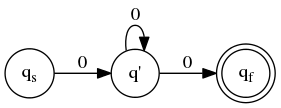
\includegraphics[width=0.3\textwidth]{assets/nfa-vb1.png}
    \caption{Een voorbeeld NFA}
    \label{fig:nfa-vb1}
  \end{figure}
\end{vb}

\begin{vb}
  Werking van bovenstaande nfa bij input string $00$:\\
  In stap $1$ kijken we naar het eerste symbool van $00$, een $0$.
  De overgangsfunctie $\delta$ zegt ons dat we met een $0$ in staat $q_{s}$ naar $q'$ kunnen gaan.
  \[ \delta(q_{s},0) = \left\{q'\right\} \]
  \begin{figure}[H]
    \centering
    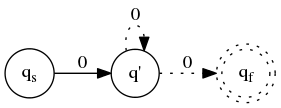
\includegraphics[width=0.3\textwidth]{assets/nfa-vb2.png}
    \caption{Stap 1}
    \label{fig:nfa-vb2}
  \end{figure}
  Het volgende symbool is opnieuw een $0$, maar nu bevindt de machine zich in staat $q'$.
  Vanuit $q'$, met een $0$ kan de automaat naar zowel $q'$ als $q_{f}$ gaan.
  Er zijn na deze stap geen symbolen meer over, de automaat stopt.
  \[ \delta(q',0) = \left\{q',q_{f}\right\} \]
  \begin{figure}[H]
    \centering
    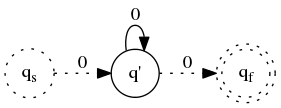
\includegraphics[width=0.3\textwidth]{assets/nfa-vb3.png}
    \caption{Stap 2.1}
    \label{fig:nfa-vb3}
  \end{figure}
  In het eerste geval eindigt de automaat in staat $q'$.
  \begin{figure}[H]
    \centering
    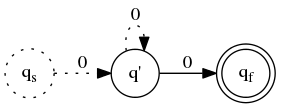
\includegraphics[width=0.3\textwidth]{assets/nfa-vb4.png}
    \caption{Stap 2.2}
    \label{fig:nfa-vb4}
  \end{figure}
  In het tweede geval eindigt de automaat in een accepterende toestand, en accepteert de automaat de string bijgevolg.
  Omdat er een opeenvolging $q_{s}q'q_{f}$ bestaat zodat de automaat de string aanvaardt, zeggen we dat de automaat de string aanvaardt.
\end{vb}

\TODO{GNFA uitvoeren}
\TODO{transitietabel}
\TODO{DFA naar NFA}
\TODO{DFA minimalisatie}
\TODO{bewijzen dat een taal niet regulier is met het pompend lemma.}

\section{Pompend lemma voor reguliere talen}
\label{sec:pompend-lemma-voor-reguliere-talen}

\begin{lem}
  Het \term{pompend lemma} voor reguliere talen\\
  Voor een \underline{reguliere} taal $L$ \underline{bestaat} er een pomplengte $d$ zodat er voor \underline{elke} string $s$ van $L$ met lengte \underline{minstens} $p$ een opdeling van $s$ \underline{bestaat} in drie stukken $x$, $y$ en $z$.
  \[ s = xyz \]
  \begin{itemize}
  \item $\forall i \in \mathbb{N}_{0}:\ xy^{i}z \in L$
  \item $|y| > 0$
  \item $|xy| \le d$
  \end{itemize}
\end{lem}
Op een iets minder formele logische manier: (Als het zo duidelijker is, kan je dit gebruiken.)
\[
\begin{array}{rrrrl}
  (\forall L\in \mathcal{P}(\Sigma^{*})) (&\\
               & Regulier(L) \Rightarrow (&\\
               &                             & (\exists p\in \mathbb{N})(&\\
               &                             &                           &(\forall s \in \Sigma^{*})(&\\
               &                             &                           &                           & (|s| \ge p)\\
               &                             &                           &                           & \Rightarrow\\
               &                             &                           &                           & (s = xyz \wedge xy^{i}z \in L)\\
               &                             &                           &                           & \text{met}\\
               &                             &                           &                           & |y| > 0 \text{ en } |xy| < p\\
               &                             &                           &                          )&\\
               &                             &                          )&\\
               &                            )&\\
              )&\\ 
\end{array}
\]

\subsection{Het pompend lemma gebruiken om te bewijzen dat een taal regulier is}
Laat dit voor eens en voor altijd duidelijk zijn:
\begin{center}
  We kunnen het pompend lemma \underline{niet} gebruiken om te bewijzen dat een taal regulier is.
\end{center}
Er bestaan immers talen met een pomplengte die niet regulier zijn.
Met andere woorden, het omgekeerde van het pompend lemma is niet waar:
\[ 
\begin{array}{c}
  L = \{ uvwxy\ |\ u,y \in \{0,1,2,3\}^{*}, v,w,x\in \{0,1,2,3\} \wedge (v=w \vee v=x \vee x=w)\}\\
  \bigcup \{ s \in \{0,1,2,3\}\ |\ \text{ precies } \frac{1}{7} \text{-de van de symbolen in } s \text{ zijn } 3 \}  
\end{array}
\]
In woorden: $L$ bevat alle strings over het alfabet $\{0,1,2,3\}$ met een substring van lengte $3$ waar een duplicaat character in zit alsook alle strings waarbij precies \'e\'en zevende van de symbolen $3$-en zijn.

\subsection{Het pompend lemma gebruiken om te bewijzen dat een taal regulier is}
We kunnen het pompend lemma \underline{wel} gebruiken om te bewijzen dat een taal \underline{niet regulier} is.
We doen dit doorgaans met een bewijs uit het ongerijmde.

Zij $L$ de taal waarvan we willen bewijzen dat hij niet regulier is.
\begin{enumerate}
\item We gaan \underline{ervan uit} dat $L$ \underline{wel} regulier is.
\item Er zou dan zeker een pomlengte $p\in \mathbb{N}$ bestaan.
\item We \underline{kiezen} \emph{heel bewust} een string $s$ langer dan $p$.
\item We tonen aan dat er \underline{geen enkele} opdeling van $s$ bestaat die aan de voorwaarden voldoet
\end{enumerate}
We hebben dan aangetoond dat er \underline{minstens \'e\'en} string $s$ bestaat die \underline{niet} gepompt kan worden, dus is de taal $L$ niet regulier.

\begin{vb}
  Bewijs dat $L = 0^{n}1^{n}$ \underline{niet} regulier is.
  \begin{proof}
    Bewijs uit het ongerijmde.
    \begin{enumerate}
    \item Stel dat $0^{n}1^{n}$ wel regulier is.
    \item Er bestaat dan zeker een pomlengte vanwege het pompend lemma.
      Noem die pomplengte $p$.
    \item We kiezen nu een string $s$ langer dan $p$:
      \[ s = 0^{p}1^{p} \]
    \item Er bestaat nu geen enkele opdeling van $s$ die aan de voorwaarden van een opdeling in het pompend lemma voldoet.
      Stel immers dat $s$ wel opgedeeld kan worden in drie stukken $xyz$, dan zijn daar drie mogelijkheden voor:
      \begin{enumerate}
      \item $y$ bevat enkel nullen.\\
        De string $xz$ bevat dan meer enen dan nullen en zit bijgevolg niet in $L$.
      \item $y$ bevat zowel nullen als enen.\\
        In de string $xyyz$ staan dan niet alle nullen voor alle enen. $xyyz$ zit dus niet in $L$. 
      \item $y$ bevat enkel enen.\\
        De string $xz$ bevat dan meer nullen dan enen en zit bijgevolg niet in $L$.
      \end{enumerate}
      Merk op dat de laatste twee mogelijkheden eigenlijk meteen geschrapt konden worden als we in rekening namen dat $xy$ korter dan $p$ moet zijn.
    \end{enumerate}
  \end{proof}
\end{vb}

\section{Pompend lemma voor contextvrije talen}
\label{sec:pompend-lemma-voor-contextvrije-talen}

\begin{lem}
  Voor een \underline{contextvrije} taal $L$ \underline{bestaat} er een pomplengte $p$  zodat er voor \underline{elke} string $s$ van $L$ met lengte \underline{minstens} $p$ een opdeling van $p$ \underline{bestaat} in vijf stukken $u$, $v$, $x$, $y$ en $z$.
  \[ s = uvxyz \]
  \begin{enumerate}
    \item $\forall i \in \mathbb{N}:\ uv^{i}xy^{i}z \in L$
    \item $|vy| > 0$
    \item $|vxy| < p$
  \end{enumerate}
\end{lem}
Op een iets minder formele logische manier: (Als het zo duidelijker is, kan je dit gebruiken.)
\[
\begin{array}{rrrrl}
  (\forall L\in \mathcal{P}(\Sigma^{*})) (&\\
               & Contextvrij(L) \Rightarrow (&\\
               &                             & (\exists p\in \mathbb{N})(&\\
               &                             &                           &(\forall s \in \Sigma^{*})(&\\
               &                             &                           &                           & (|s| \ge p)\\
               &                             &                           &                           & \Rightarrow\\
               &                             &                           &                           & (s = uvxyz \wedge uv^{i}xy^{i}z \in L)\\
               &                             &                           &                           & \text{met}\\
               &                             &                           &                           & |vy| > 0 \text{ en } |vxy| < p\\
               &                             &                           &                          )&\\
               &                             &                          )&\\
               &                            )&\\
              )&\\ 
\end{array}
 \]

\subsection{Het pompend lemma gebruiken om te bewijzen dat een taal contextvrij is}
Laat dit ook voor eens en voor altijd duidelijk zijn:
\begin{center}
  We kunnen het pompend lemma \underline{niet} gebruiken om te bewijzen dat een taal contextvrij is.
\end{center}
Er bestaan immers talen met een pomplengte die niet contextvrij zijn.
\extra{tegenvoorbeeld voor het omgekeerde van het pompend lemma voor contextvrije talen}

\subsection{Het pompend lemma gebruiken om te bewijzen dat een taal contextvrij is}
We kunnen het pompend lemma \underline{wel} gebruiken om te bewijzen dat een taal \underline{niet contextvrij} is.
We doen dit doorgaans ook met een bewijs uit het ongerijmde.

Zij $L$ de taal waarvan we willen bewijzen dat hij niet contextvrij is.
\begin{enumerate}
\item We gaan \underline{ervan uit} dat $L$ \underline{wel} contextvrij is.
\item Er zou dan zeker een pomlengte $p\in \mathbb{N}$ bestaan.
\item We \underline{kiezen} \emph{heel bewust} een string $s$ langer dan $p$.
\item We tonen aan dat er \underline{geen enkele} opdeling van $s$ bestaat die aan de voorwaarden voldoet
\end{enumerate}
We hebben dan aangetoond dat er \underline{minstens \'e\'en} string $s$ bestaat die \underline{niet} gepompt kan worden, dus is de taal $L$ niet contextvrij.

\begin{vb}
  Bewijs dat $0^{n}1^{n}2^{n}$ \underline{niet} contextvrij is.
  \begin{proof}
    Bewijs uit het ongerijmde.
    \begin{enumerate}
    \item Stel dat $L = 0^{n}1^{n}2^{n}$ wel contextvrij is.
    \item Er bestaat dan zeker een pomplengte vanwege het pompend lemma.
      Noem die pomplengte $p$.
    \item We kiezen nu een string $s$ langer dan $p$:
      \[ s = 0^{p}1^{p}2^{p} \]
    \item Er bestaat nu geen enkele opdeling van $s$ die aan de voorwaarden voldoet.
      Stel immers dat $uvxyz$ wel een geldige opdeling van $s$ is met $|vy| > 0$ en $|vxy| < p$.
      Er zijn dan twee mogelijkheden:
      \begin{enumerate}
      \item $v$ en $y$ bevatten elk hoogstens \'e\'en verschillend symbool.
        $v$ is dan van de vorm $\alpha^{k}$ en $y$ is van de vorm $\beta^{l}$ waarbij $\alpha$ en $\beta$ beide $0$ $1$ of $2$ zijn. 
        $k+l$ is bovendien groter dan nul want $|vy| > 0$ moet gelden.
        De string $uv^{2}xy^{2}z$ kan dan al niet bestaan uit een gelijk aantal nullen, enen en twe\"en.
        $uv^{2}xy^{2}z$ zit dan dus niet in $L$.
      \item $v$ of $y$ bevat meer dan \'e\'en verschillend symbool.
        In de string $uv^{2}xy^{2}z$ staan de symbolen in $v^{2}$ of in $y^{2}$ dan niet in de juiste volgorde.
        $uv^{2}xy^{2}z$ zit dan bijgevolg niet in $L$.
      \end{enumerate}
    \end{enumerate}
  \end{proof}
\end{vb}







\TODO{encoderingen}

\end{document}

